\documentclass[11pt,a4paper]{article}

\usepackage[utf8]{inputenc} 
\usepackage[T1]{fontenc} 
\usepackage{lmodern}
\usepackage[margin=2cm]{geometry}
\usepackage[german]{babel}
\usepackage{amsmath} 
\usepackage{graphicx} 
\usepackage{booktabs}
\usepackage{hyperref}
\usepackage{gensymb}
\hypersetup{
    colorlinks,
    citecolor=red,
    filecolor=black,
    linkcolor=black!20!blue!90!,
    urlcolor=black} 
\usepackage{nicefrac}
\usepackage[table]{xcolor}
\usepackage{tocloft}

\setlength{\parindent}{0pt}
\setlength{\parskip}{1ex plus 0.5ex minus 0.5ex}

\definecolor{incolor}{rgb}{0.0, 0.0, 0.5}

\hbadness=99999

\newcommand{\refpy}[1]{Siehe Anhang: \textit{Rechnungen in Python} (\texttt{{\color{incolor}In [{\color{incolor}#1}]}})}
\newcommand\dif{\mathop{}\!\mathrm{d}}
\newcommand{\halftime}[4]{\begin{figure}[h]
\begin{minipage}{.#1\textwidth}#3\end{minipage}\begin{minipage}{.#2\textwidth}
\centering
#4\end{minipage}
\end{figure}}
\renewcommand{\vec}{\boldsymbol}

\begin{document}

% name of experiment
% date of experiment
% name of assistant
{
\centering 
\large 
Physiklabor für Anf\"anger*innen \\
Ferienpraktikum im Sommersemester 2018 \\[4mm]
\textbf{\LARGE 
Versuch 23: Schallwellen
} \\[3mm]
(durchgef\"uhrt am 08.10.2018 bei Pascal Wunderlin) \\
Ye Joon Kim (Gruppe 13), Patrick M\"unnich (Gruppe 14)\\
\today \\[10mm]
}

\vspace{50pt}
\tableofcontents
\vspace{22pt}
\listoftables
\vspace{22pt}
\listoffigures
\pagebreak

\section{Ziel des Versuchs}
Das Ziel dieses Versuchs ist es, die Schallschallgeschwindigkeit von Luft auf drei Weisen zu bestimmen. 

\section{1. Versuchsteil: Bestimmung der Schallgeschwindigkeit mit einem Quinckeschen Rohr}


\subsection{Aufbau}

\begin{figure}
	\centering
	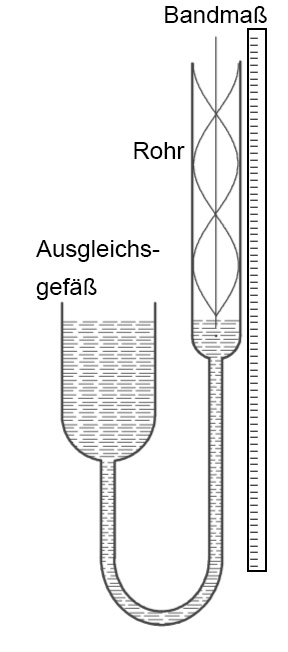
\includegraphics[scale=0.5]{Abb1}
	\caption{Aufbau zum ersten Versuchsteil: Ein quinckeschen Rohr. \cite{Anleitung}}
\end{figure}
Für den ersten Versuchsteil wurde ein Quinckesches Resonanzrohr verwendet (Siehe Abbildung 1). \"Uber dem linken Rohr sind ein Mikrofon und ein Lautspricher zu finden. Diese sind jeweils an ein Oszilloskop und ein Frequenzgenerator gebunden.

% describe set up
% insert pic name, designation, toc caption, caption, label
%\halftime{5}{5}{TEXT}{\fbox{\includegraphics[width=0.5\textwidth]{NAME}}
%   \renewcommand\thefigure{BX}
%\caption[XXXX]{XXXX \cite{Anleitung}}
%\label{Pic:X}}

\subsection{Durchführung}
Die Frequenzgenerator und der Oszillator wurden angeschaltet. Es wurde dann eine Frequenz zwischen 2\,kHz und 7\,kHz ausgewählt. Die Wasserhöhe in dem Rohr wurde dann verkleinert, indem man das Ausgleichsgefäß senkt. Sobald eine maximale Amplitude in dem Oszilloskop beobachtet wurde, wurde die Höhe des Wasserspiegels in dem Rohr mit einem Maßband gemessen. Dies wurde auch gemessen, als ein Minimum beobachtet wurde. Für jede Frequenz wurden die Wasserhöhe für 8-10 Maxima und Minima gemessen. Es wurden drei Unterschiedliche Frequenzen untersucht. 


\subsection{Auswertung und Fehleranalyse}

Um mit unseren Messdaten die Schallgeschwindigkeit bestimmen zu k\"onnen, tragen wir zuerst die Lagen der Maxima und Minima in Diagramme auf. Daraufhin f\"uhren wir eine lineare Regression durch und f\"ugen sie dem Bild hinzu. Die Resultierenden Graphiken k\"onnen im Anhang als Abbildung \ref{Abb:4}, \ref{Abb:5} und \ref{Abb:6} gefunden werden.

Um die lineare Regression durchf\"uhren zu k\"onnen, nehmen wir uns das folgende Polynom ersten Grades vor:
\[ a+bx\]

F\"ur $a$ berechnen wir

\[a=\frac{\sum x_i^2\sum y_i-\sum x_i\sum x_iy_i}{n\sum x_i^2-(\sum x_i)^2}\]
und f\"ur b
\[b=\frac{n\sum x_iy_i-\sum x_i\sum y_i}{n\sum x_i^2-(\sum x_i)^2}.\]

Wollen wir die Unsicherheiten bestimmen, so k\"onnen wir die folgenden Formeln verwenden:
\[
s=\sqrt{\frac{1}{n-2}\sum^n_{i=1}[y_i-(a+bx_i)]^2}\]

\[\Delta a=s\sqrt{\frac{\sum x_i^2}{n\sum x_i^2-(\sum x_i)^2}}\]

\[\Delta b=s\sqrt{\frac{n}{n\sum x_i^2-(\sum x_i)^2}}\]

Mit diesen Formeln erhalten wir als Werte

\begin{table}[h]
	\centering
	\begin{tabular*}{0.50\textwidth}{@{\extracolsep{\fill}}cccc}
		\toprule
		Messreihe & $b$ & $u_b$ \\
		& cm & cm\\
		1 & 4,5 & 0,3\\
		2 & 7,6 & 0,3\\
		3 & 4,5 & 0,3\\
		\bottomrule
	\end{tabular*}
\caption{Die berechneten Steigungen der linearen Regressionen von $\nu$ gegen $l$}
\label{Table1}
\end{table}

Wir nutzen dann die Steigung, um die Wellenl\"angen zu bestimmen. Wir berechnen dann einfach mit
\begin{equation}
c=\nu\lambda
\end{equation}
die Ausbreitungsgeschwindigkeit der Wellen.
Die einzelnen Werten wurden dann gemittelt, und ihre Standardabweichung wurde berechnet, um die Standardunsicherheit:
$$u_{\bar{c}} = \frac{1}{\sqrt{n}} \sqrt{\frac{\sum_{i=1}^{n}(c_i-\bar{c})^2}{n-1}}$$
des Mittelwerts zu berechnen. 
 
Das Ergebnis lautet dann:
$$ c= (370 \pm 60)\,\nicefrac{\mathrm{m}}{\mathrm{s}}$$








\section{Diskussion der Ergebnisse}

Um einen Vergleichwert zu erhalten, rechnen wir mit

\[
c_l=331\left(\sqrt{\frac{T}{273,15\mathrm{K}}}\right)\frac{\mathrm{m}}{\mathrm{s}}\approx\left(331+0,6\frac{\Delta T}{\mathrm{K}}\right)\mathrm{\frac{m}{s}}
\]

den theoretischen Wert f\"ur die Schallgeschwindigkeit in dem verwendeten Raum. In diesem Fall wurde $T=23$\celsius\ verwendet, und wir erhalten somit als Vergleichswert:

\[
c = 344\,\nicefrac{\mathrm{m}}{\mathrm{s}}
\]

Um zu sehen, ob der theoretische und die gemessenen Werte miteinander verträglich sind, wurde ihre Differenz in Einheiten der Unsicherheit, $t = \frac{c-c\textrm{theo}}{u_c}$ berechnet: 
$$t_c = 0,43$$
Da also $t<2$, sind die beiden Werte miteinander verträglich. Das Problem ist aber, dass die relative Unsicherheit des gemessenen Werts ungefähr 16\% beträgt. Deshalb ist dieses Ergebnis nicht besonders signifikant.

Ein sehr signifikanter statistischer Fehler war es, dass es sehr schwierig war, die genaue Lage des Maximums oder Minimums zu bestimmen, da die Schwankungen sehr graduell waren. Bei größeren Wellenlänge sind die Messungen noch schwieriger. Dieses Problem lässt sich lösen, indem man einen Oszilloskop benutzt, das besser die Amplitude und die Welle selbst darstellen kann. 

\pagebreak

\section{2. Versuchsteil: Bestimmung der Ultraschallgeschwindigkeit durch die Messung der Wellenlänge.}
\subsection{Aufbau}
\begin{figure}
	\centering
	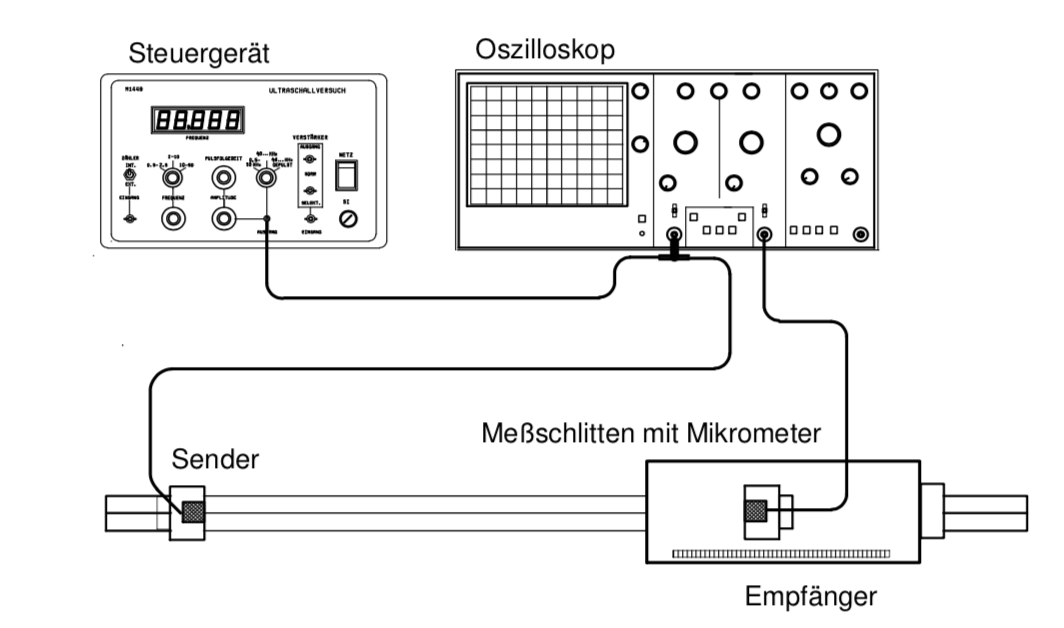
\includegraphics[scale=0.5]{Abb2}
	\caption{Aufbau zum zweiten Versuchsteil. \cite{Anleitung}}
\end{figure}

Für diesen Versuchsteil wurden ein Ultraschallsender und -empfänger, ein Oszilloskop, ein Signalgenerator und eine Mikrometerschraube verwendet (siehe Abbildung 2). Sender und Empf\"anger werden an das Oszilloskop (und Sender auch an das Steuerger\"at) angeschlo\ss en. Die beiden werden dann auf beide Enden der Bank gestellt, sodass sie auf einander zeigen.

\subsection{Durchführung}
Der Sender und der Empfänger (mit der Mikrometerschraube) wurden auf beiden Seiten der Bank fixiert. Der Oszilloskop wurde angeschaltet und justiert, sodass beide Signale im Bildschirm zu sehen waren. Der Empfänger wurde dann mit der Mikrometerschraube verschoben, sodass die zwei angezeigten Signale in Deckung waren. Seine Position relativ zur Mikrometerschraube wurde dann aufgenommen. Der Empfänger wurde daraufhin wiederum mit dem Mikrometerschraube verschoben, bis die zwei Signale wieder in Deckung waren. Seine Position wurde dann wieder aufgenommen. Die Positionen wurden 10-mal für jedes mal, dass die zwei Signalen in Deckung waren, gemessen. Dieser Prozess wurde für vier verschiedene Startpositionen des Empfängers wiederholt. 



\subsection{Auswertung und Fehleranalyse}
Für jede Messreihe wurden die $x$ Werte gegen $k$ aufgetragen (siehe Anhang). Die linearen Regressionen wurden mithilfe eines Excel-Dokuments mit den folgenden Formel berechnet: 

Die Steigung $b$ ist:
$$ b = \frac{n\sum k_ix_i-\sum k_i \sum x_i}{n \sum k_i^2 - (\sum k_i)^2}$$

und ihre Unsicherheit:
$$u_b = s\cdot \sqrt{\frac{n}{n\sum k_i^2 - (\sum k_i)^2}}$$
Mit 
$s = \sqrt{\frac{1}{n-2}\sum [x_i-(a+bk_i)]^2}$

Es wurden nur die Steigungen und deren Unsicherheiten berechnet, da der Achsenabschnitt irrelevant zum erw\"unschten Ergebnis ist. Die berechneten Steigungen und deren Unsicherheiten für jede Messreihe sind in Tabelle \ref{Table1} zu sehen. 


\begin{table}[h]
	\centering
	\begin{tabular*}{0.50\textwidth}{@{\extracolsep{\fill}}cccc}
		\toprule
		Messreihe & $b$ & $u_b$ \\
		& cm & cm\\
		1 & 9,1 & 1,7 \\
		2 & 8,6 & 0,2 \\
		3 & 8,46 & 0,15 \\
		4 & 8,51 & 0,02 \\
		\bottomrule
	\end{tabular*}
\caption{Die berechneten Steigungen der linearen Regressionen von $x$ gegen $k$}
\label{Table1}
\end{table}

Um die Schallgeschwindigkeit zu bestimmen wurde die folgende Formel benutzt:
$$ c = \nu\lambda$$

Für $\nu$ wurde die durchschnittliche Frequenz während der Messreihe benutzt. Seine Unsicherheit wurde mit der Standardunsicherheit berechnet, nämlich:
$$ u_\nu = \frac{s_\nu}{\sqrt{n}}$$
und
$$ s_{\bar{\nu}} = \sqrt{\frac{\sum_{i=1}^{n}(\nu_i-\bar{\nu})^2}{n-1}}.$$

Für die Unsicherheiten der Schallgeschwindigkeiten wurde die vereinfachte gaußsche Fehlerfortpflanzung für Produkte benutzt, aber da die Beträge von $\frac{u_\lambda}{\lambda}$ rund 100-mal größer als die von den $\frac{u_\nu}{\nu}$ Terme waren, wurde die Letzteren vernachlässigt. Die Unsicherheit von $c$ ist deshalb:
$$ u_c = \left| \frac{u_\lambda}{\lambda}\right|$$

Die berechnete Werte für die Schallgeschwindigkeiten und ihre Unsicherheiten sind in Tabelle \ref{Table2} zu sehen.

\begin{table}[h]
	\centering
	\begin{tabular*}{0.50\textwidth}{@{\extracolsep{\fill}}cccc}
		\toprule
		Messreihe & $c$ & $u_c$ \\
		& m/s&m/s\\
		1 & 370 & 70 \\
		2 & 350 & 10 \\
		3 & 342 & 6 \\
		4 & 344,2 & 0,8 \\
		\bottomrule
	\end{tabular*}
	\caption{Die berechnete Schallgeschwindigkeit für alle Messreihe}
\label{Table2}
\end{table}

Die $c$ Werte wurden gemittelt und ihre Standardunsicherheit berechnet. 

$$ c = (351 \pm 6)\,\nicefrac{\mathrm{m}}{\mathrm{s}}$$

Die Unsicherheit wurde genau wie oben mit
$$u_{\bar{c}} = \frac{1}{\sqrt{n}} \sqrt{\frac{\sum_{i=1}^{n}(c_i-\bar{c})^2}{n-1}}$$
berechnet. 




\subsection{Diskussion der Ergebnisse}


Die mit der Wellenlängemessung bestimmte Schallgeschwindigkeit ist:
$$ c = (351 \pm 6)\,\nicefrac{\mathrm{m}}{\mathrm{s}}$$

Um zu sehen, ob dieses Ergebnis und der theoretischer Wert miteinander verträglich sind, wurde ihre Differenz in Einheiten der Standardunsicherheit berechnet, nämlich mit:
$$ t = \frac{c - c_\textrm{theo}}{u_{\bar{c}}}, $$
 was $t \approx 1,03 $ beträgt. 
	
Da dieser Wert kleiner als 2 ist, sind die zwei Werte miteinander verträglich, und da die relative Unsicherheit 1,7\% ist, ist dieses Ergebnis auch signifikant. 

Ein statistischer Fehler war es, dass die Auflösung und Größe des Bildschirms nicht besonders gut waren. Deswegen war es ein Bisschen schwierig festzustellen, ob beide Wellen genau in Deckung waren. Dieses Problem lässt sich dadurch lösen, dass man ein Oszilloskop mit einem größeren Bildschirm oder besserer Auflösung benutzt. 

Ein anderer Fehler war es, dass die abgebildeten Wellen nach der Zeit sich leicht verschoben, obwohl die ,,Trigger'' Funktion benutzt wurde. Sein Einfluss wurde minimiert, indem man die Lage der gesamten Abbildung ständig horizontal mit dem Drehknopf korrigiert. 





\section{3. Versuchsteil: Bestimmung der Ultraschallgeschwindigkeit durch die Messung der Laufzeit}

\subsection{Aufbau}
\begin{figure}[h]
	\centering
	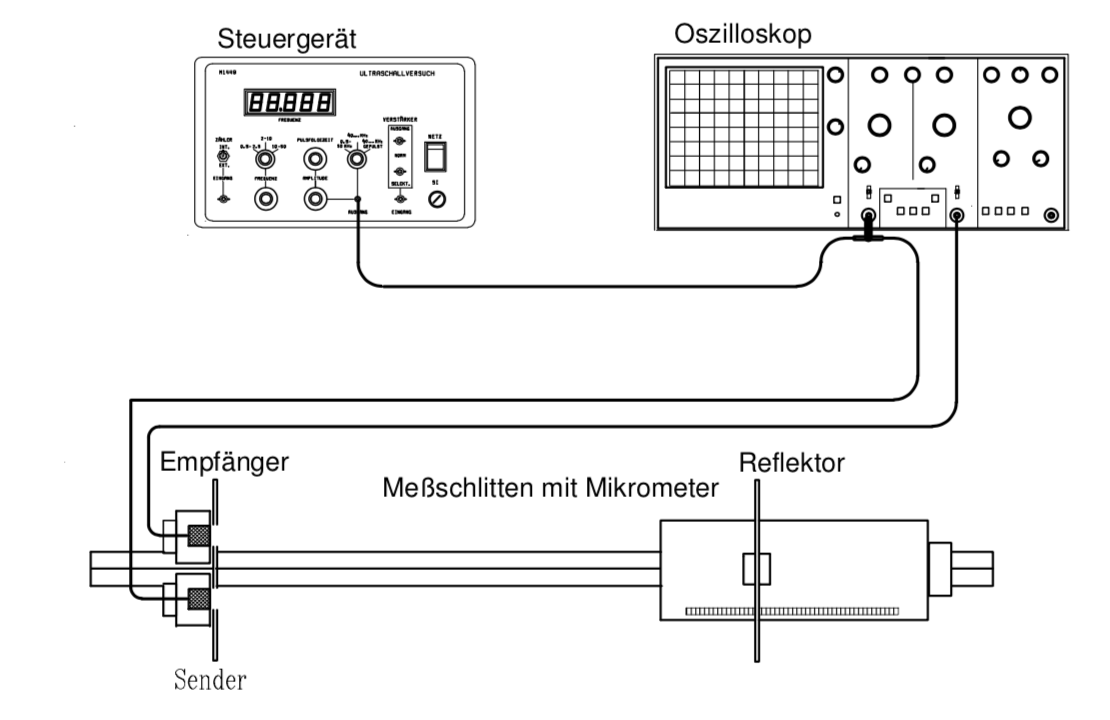
\includegraphics[scale=0.5]{Abb3}
	\caption{Aufbau zum dritten Versuchsteil. \cite{Anleitung}}
\end{figure}
Für diesem Versuchsteil wurden dieselben Apparate wie in dem zweiten Teil und ein Reflektor benutzt (siehe Abbildung 3). Der Unterschied in diesem Teil ist, dass wir Empf\"anger und Sender parallel nebeneinander setzten und in der Position wo vorher unser Empf\"anger war einen Reflektor setzen.

\subsection{Durchführung}
Zu diesem Versuchsteil wurdne der Empfänger und der Sender auf derselben Seite der Bank fixiert. Auf der anderen Seite wurde ein Reflektor installiert. Es wurde die Betriebsart 3 des Frequenzgenerators ausgewählt. Das Oszilloskop und der Frequenzgenerator wurden angeschalten und justiert, sodass zwei Pulse im Bildschirm des Oszilloskops zu sehen waren. Der Abstand zwischen dem Empfänger-Sender Komplex und dem Reflektor wurde mit einem Maßband gemessen. Der Zeitdauer zwischen dem ausgesandten Puls und empfangenen Puls wurde direkt mithilfe der Skala auf dem Oszilloskop gemessen. 

\subsection{Auswertung und Fehleranalyse}

Um die Schallgeschwindigkeit zu bestimmen, tragen wir unsere gemessenen Daten mit $t$ gegen $x$ auf und f\"uhren eine lineare Regression durch.  Das Resultat kann im Anhang als Abbildung \ref{Abb:8} gefunden werden.

Wir erhalten mit der in den vorherigen Teil beschriebenen Methode f\"ur unsere Steigung einen Wert von 188,72\,$\nicefrac{\mathrm{m}}{\mathrm{s}}$. Da wir nur eine halbe Wellenl\"ange messen, verdoppeln wir diesen Wert und erhalten eine Schallgeschwindigkeit von 

\[
377,44\,\nicefrac{\mathrm{m}}{\mathrm{s}}.
\]

Um die Unsicherheit des Wertes zu bestimmen sollen wir mit der Formel f\"ur die Streuung,

\[s_x=\sqrt{\frac{1}{n-1}\sum_{i=1}^n(x_i-\overline{x})^2},\]

 die Unsicherheit berechnen und erhalten 0,09\,$\nicefrac{\mathrm{m}}{\mathrm{s}}$.

Berechnen wir aber mit der Formel f\"ur die Unsicherheit von Steigung bei linearer Regression die Unsicherheit, so bekommen wir als Wert
\[
0,03\,\nicefrac{\mathrm{m}}{\mathrm{s}}
\]

\subsection{Diskussion}

Vergleichen wir diesen Wert mit dem mit Streuung berechneten Fehler mit der schon bekannten $t$-Formel

\[\frac{\vert x-y_0\vert}{u_x}\]

mit dem vorher berechneten theoretischen Ergebniss, so erhalten wir $t=1626$. Wir sind hiermit also deutlich au\ss erhalb des erw\"unschten $t>2$-Bereichs. Daraus schlie\ss en wir, dass unsere Werte unvertr\"aglich sind.

Mit dem Wert mit dem Fehler aus der Steigung erhalten wir $t=5143$. Daraus schlie\ss en wir das Selbe wie mit dem vorherigen Fehler.

Um dieses Ergebnis verstehen zu k\"onnen, muss klar gemacht werden, dass durch die Zeitablenkung des Oszilloskops eine systematische Unsicherheit vorhanden ist. Es kann also sein, dass das Oszilloskop falsch eingestellt wurde und somit jede Messung einzeln eine andere systematische Unsicherheit aufgrund der Neueinstellung des Ger\"ats besitzt.

Au\ss erdem ist gleich wie beim vorherigen Teil auch das Ablesen des Messwertes ungenau. Durch Schwierigkeiten des Ablesens bei kleinen Gitterlinien haben wir eine statistische Unsicherheit auf der Zeit. Ist die Unsicherheit hiervon falsch gesch\"atzt, so beeinflusst dies unsichere Steigung stark.

Es gelten dieselben Verbesserungsvorschläge wie in dem zweiten Versuchsteil. 

\pagebreak

\section{Zusammenfassung}

Mit unseren drei verschiedenen Weisen haben wir folgende Werte f\"ur die Schallgeschwindigkeit bestimmt:

\begin{table}[h]
	\centering
	\begin{tabular*}{0.50\textwidth}{@{\extracolsep{\fill}}ccccc}
		\toprule
		Messweise & $c$ & $u_c$ & t\\
		& m/s&m/s &\\
		1 & 370 & 60 & 0,43 \\
		2 & 351 & 6 & 1,03\\
		3 & 377,44 & 0,09 bzw. 0.03, & 1626 bzw. 5143\\
		Theorie & 344,2 & \\
		\bottomrule
	\end{tabular*}
	\caption{Zusammenfassung der Endergebnisse}
\label{Table3}
\end{table}

Wir k\"onnen also erkennen, dass die letzte Messweise stark von dem Theoretischen Wert abweicht und mit den anderen Weiten schlecht \"ubereinstimmt.

Betrachten wir also die ersten beiden Experimente, so sehen wir, dass beide innerhalb des 2-$\sigma$ Bereichs liegen, wobei bei der ersten Messung der $t$ Wert deutlich kleiner ist als bei der zweiten. Jedoch ist der Fehler bei der ersten Messung 16\% des Wertes und bei der zweiten Messung 1,7\%.

Also sind zwar beide der ersten Messweisen mit der Theorie vertr\"aglich, jedoch ist die erste nicht signifant. Wir folgern daraus, dass das zweite Experiment der experimentellen Bestimmung der Schallgeschwindigkeit besser dient.



\section{Anhang: Tabellen und Diagramme}


\begin{figure}[p]
\centering
\fbox{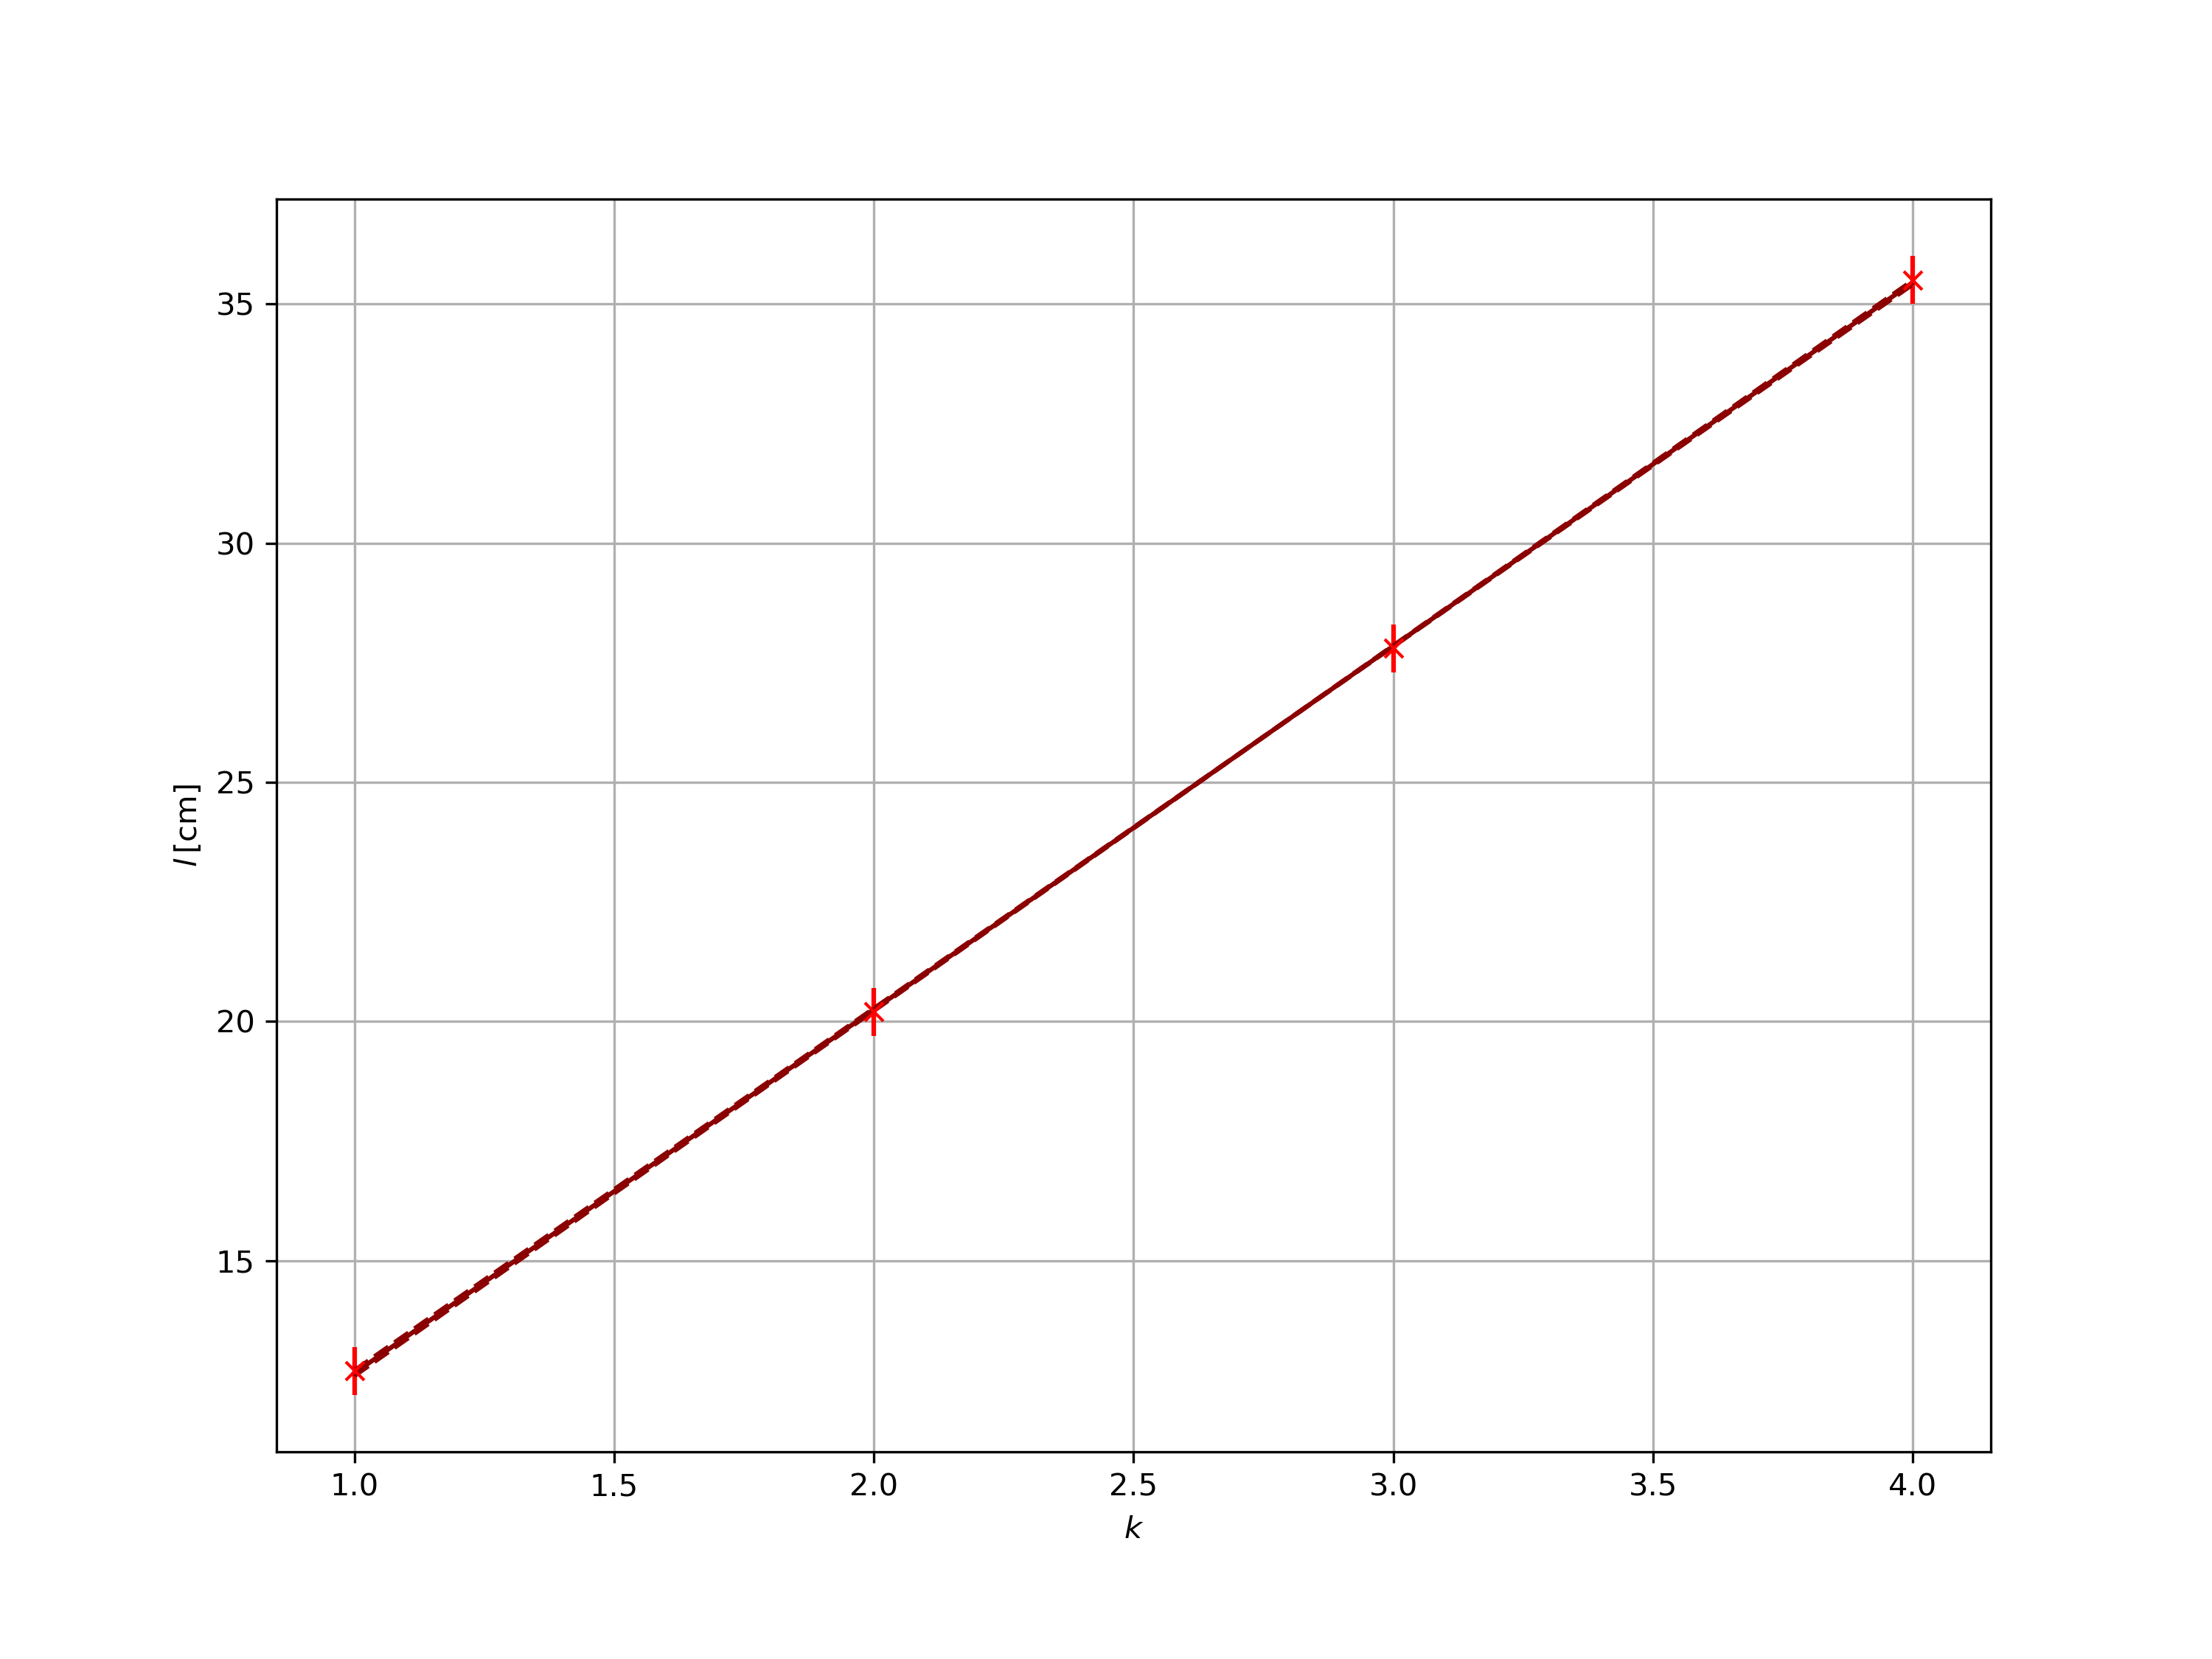
\includegraphics[width=0.8\textwidth]{1minimumonnly}}
\renewcommand\thefigure{4}
\caption[Auftragen der Minima in Abh\"angikeit der Frequenz f\"ur den ersten Versuchsteil]{Auftragen der Minima in Abh\"angikeit der Frequenz f\"ur den ersten Versuchsteil. Frequenz ist hier circa 3612\,Hz}
\label{Abb:4}
\end{figure}


\begin{figure}[p]
\centering
\fbox{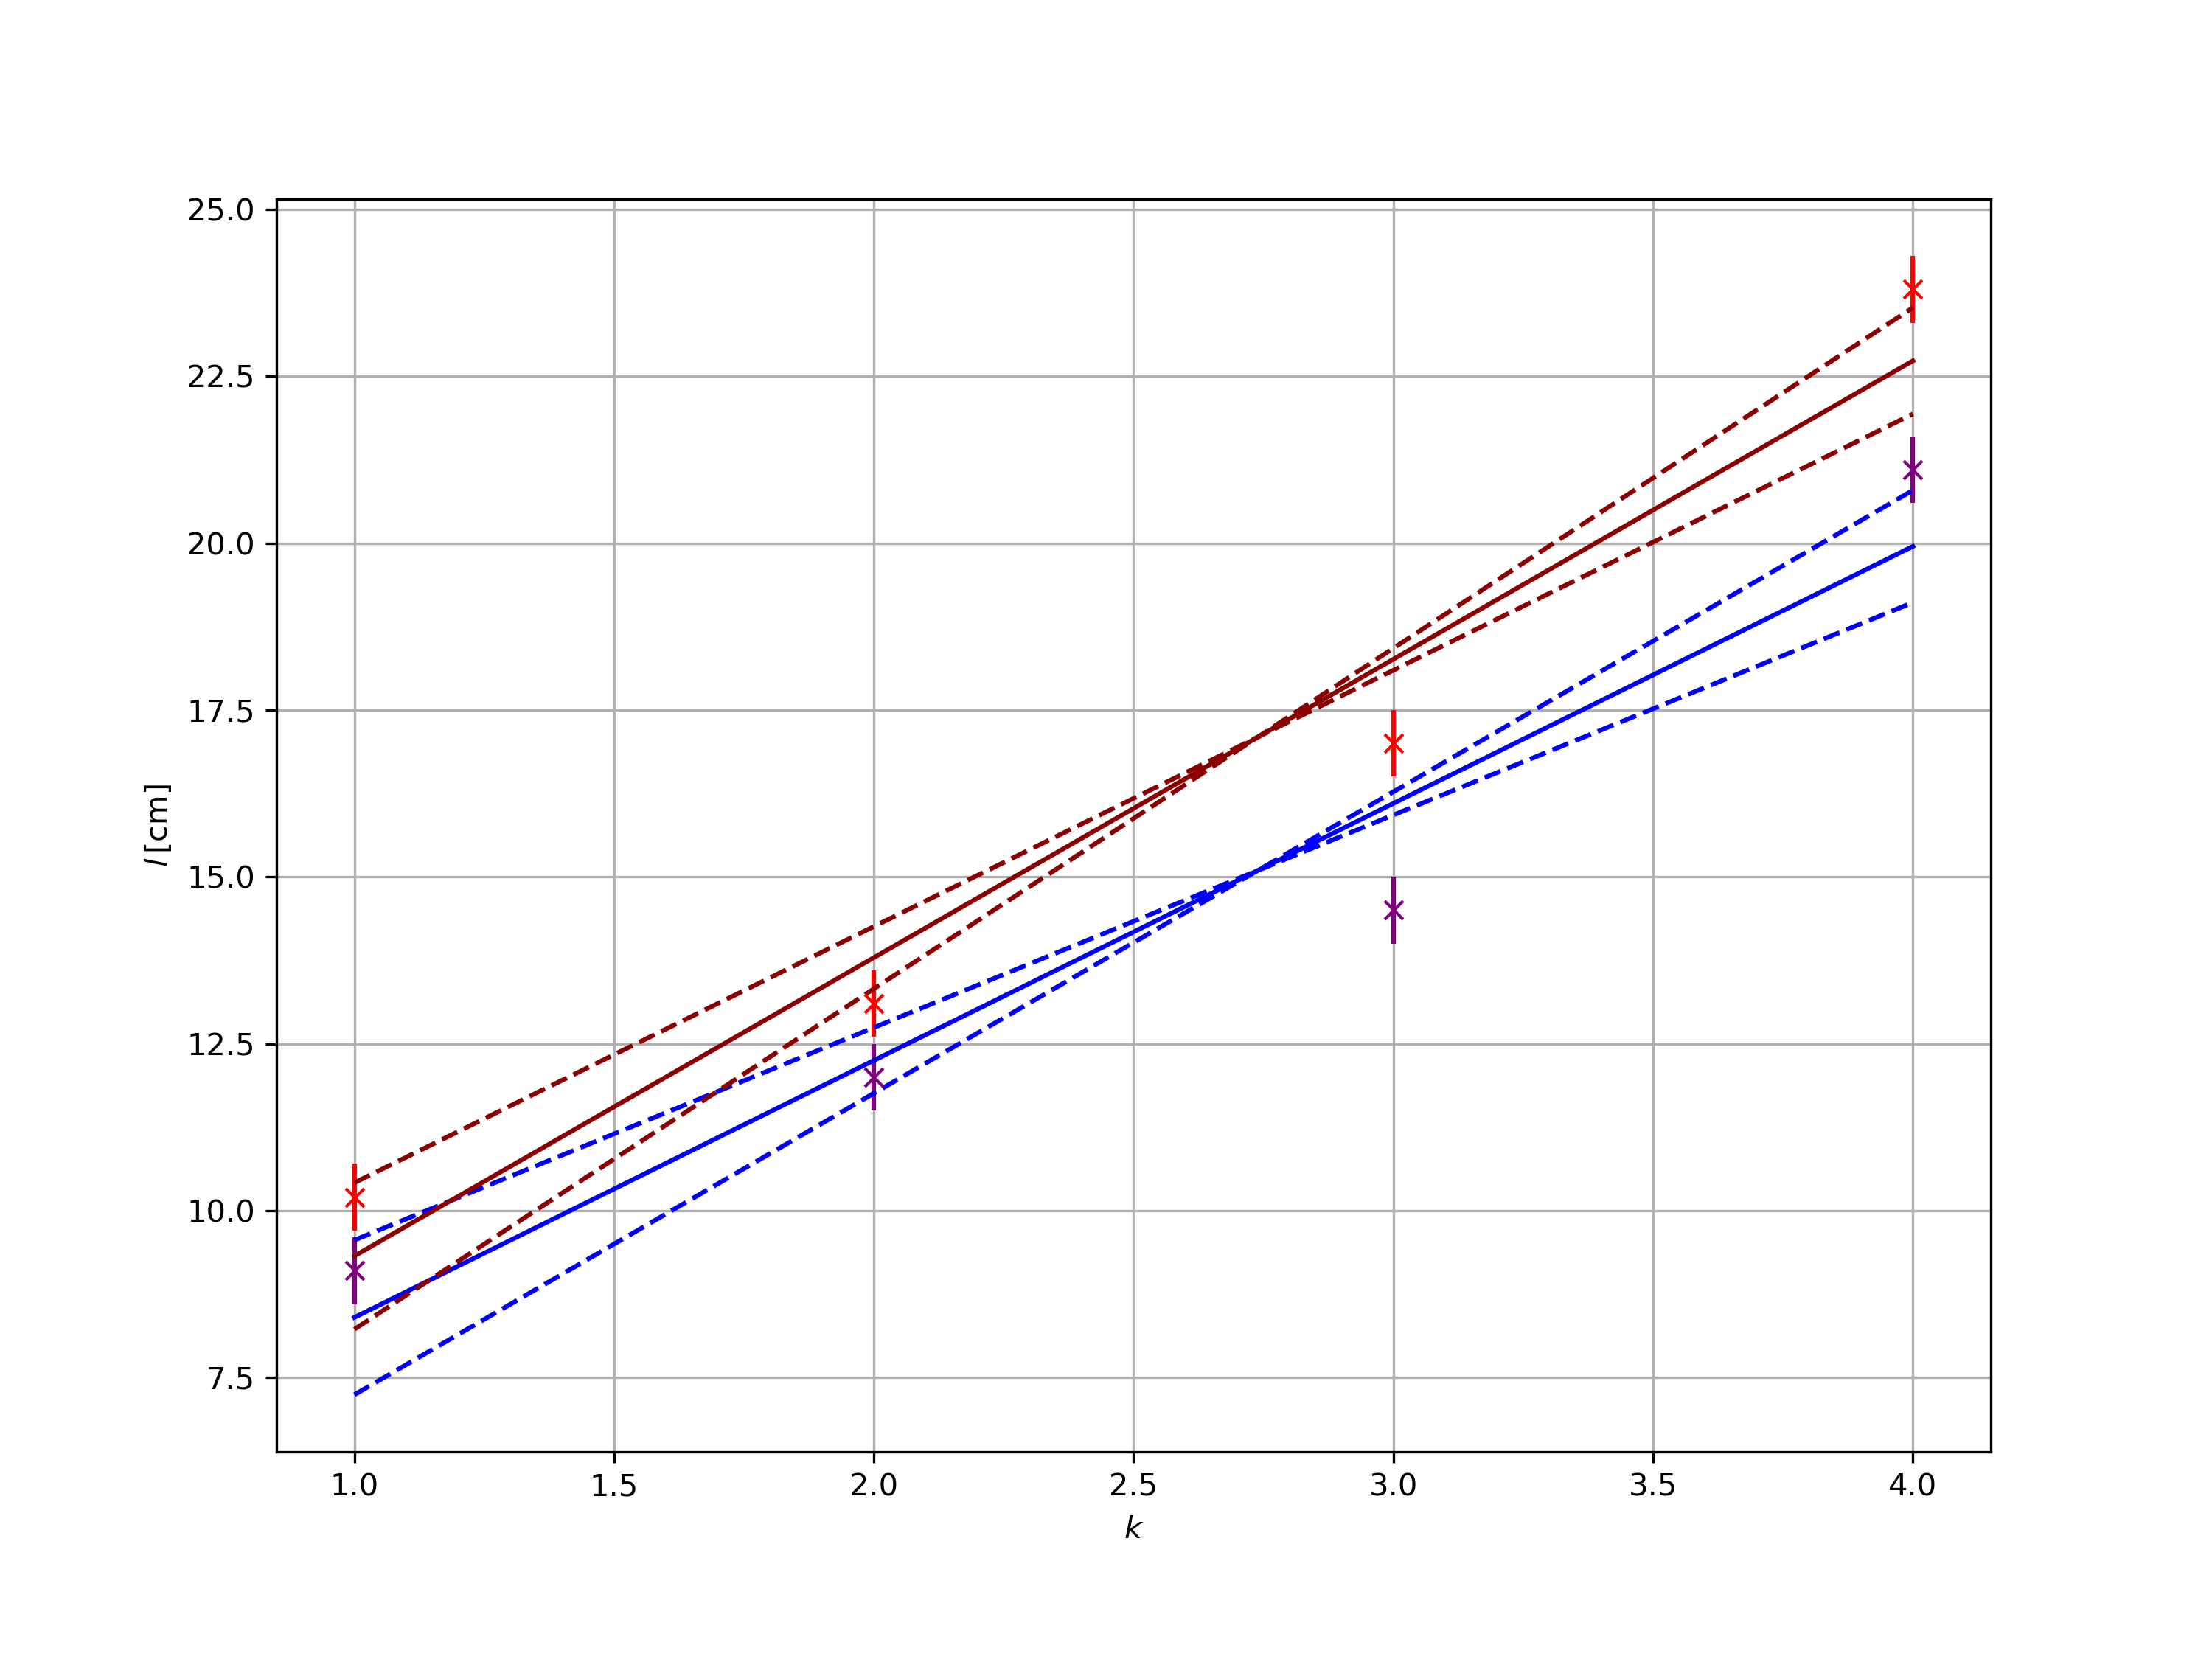
\includegraphics[width=0.8\textwidth]{1secondmeasurementminmax}}
\renewcommand\thefigure{5}
\caption[Auftragen der Maxima und Minima in Abh\"angikeit der Frequenz f\"ur den ersten Versuchsteil bei Frequenz um 5036 Hz]{Auftragen der Maxima und Minima in Abh\"angikeit der Frequenz f\"ur den ersten Versuchsteil bei Frequenz um 2263\,Hz.}
\label{Abb:5}
\end{figure}

\begin{figure}[p]
\centering
\fbox{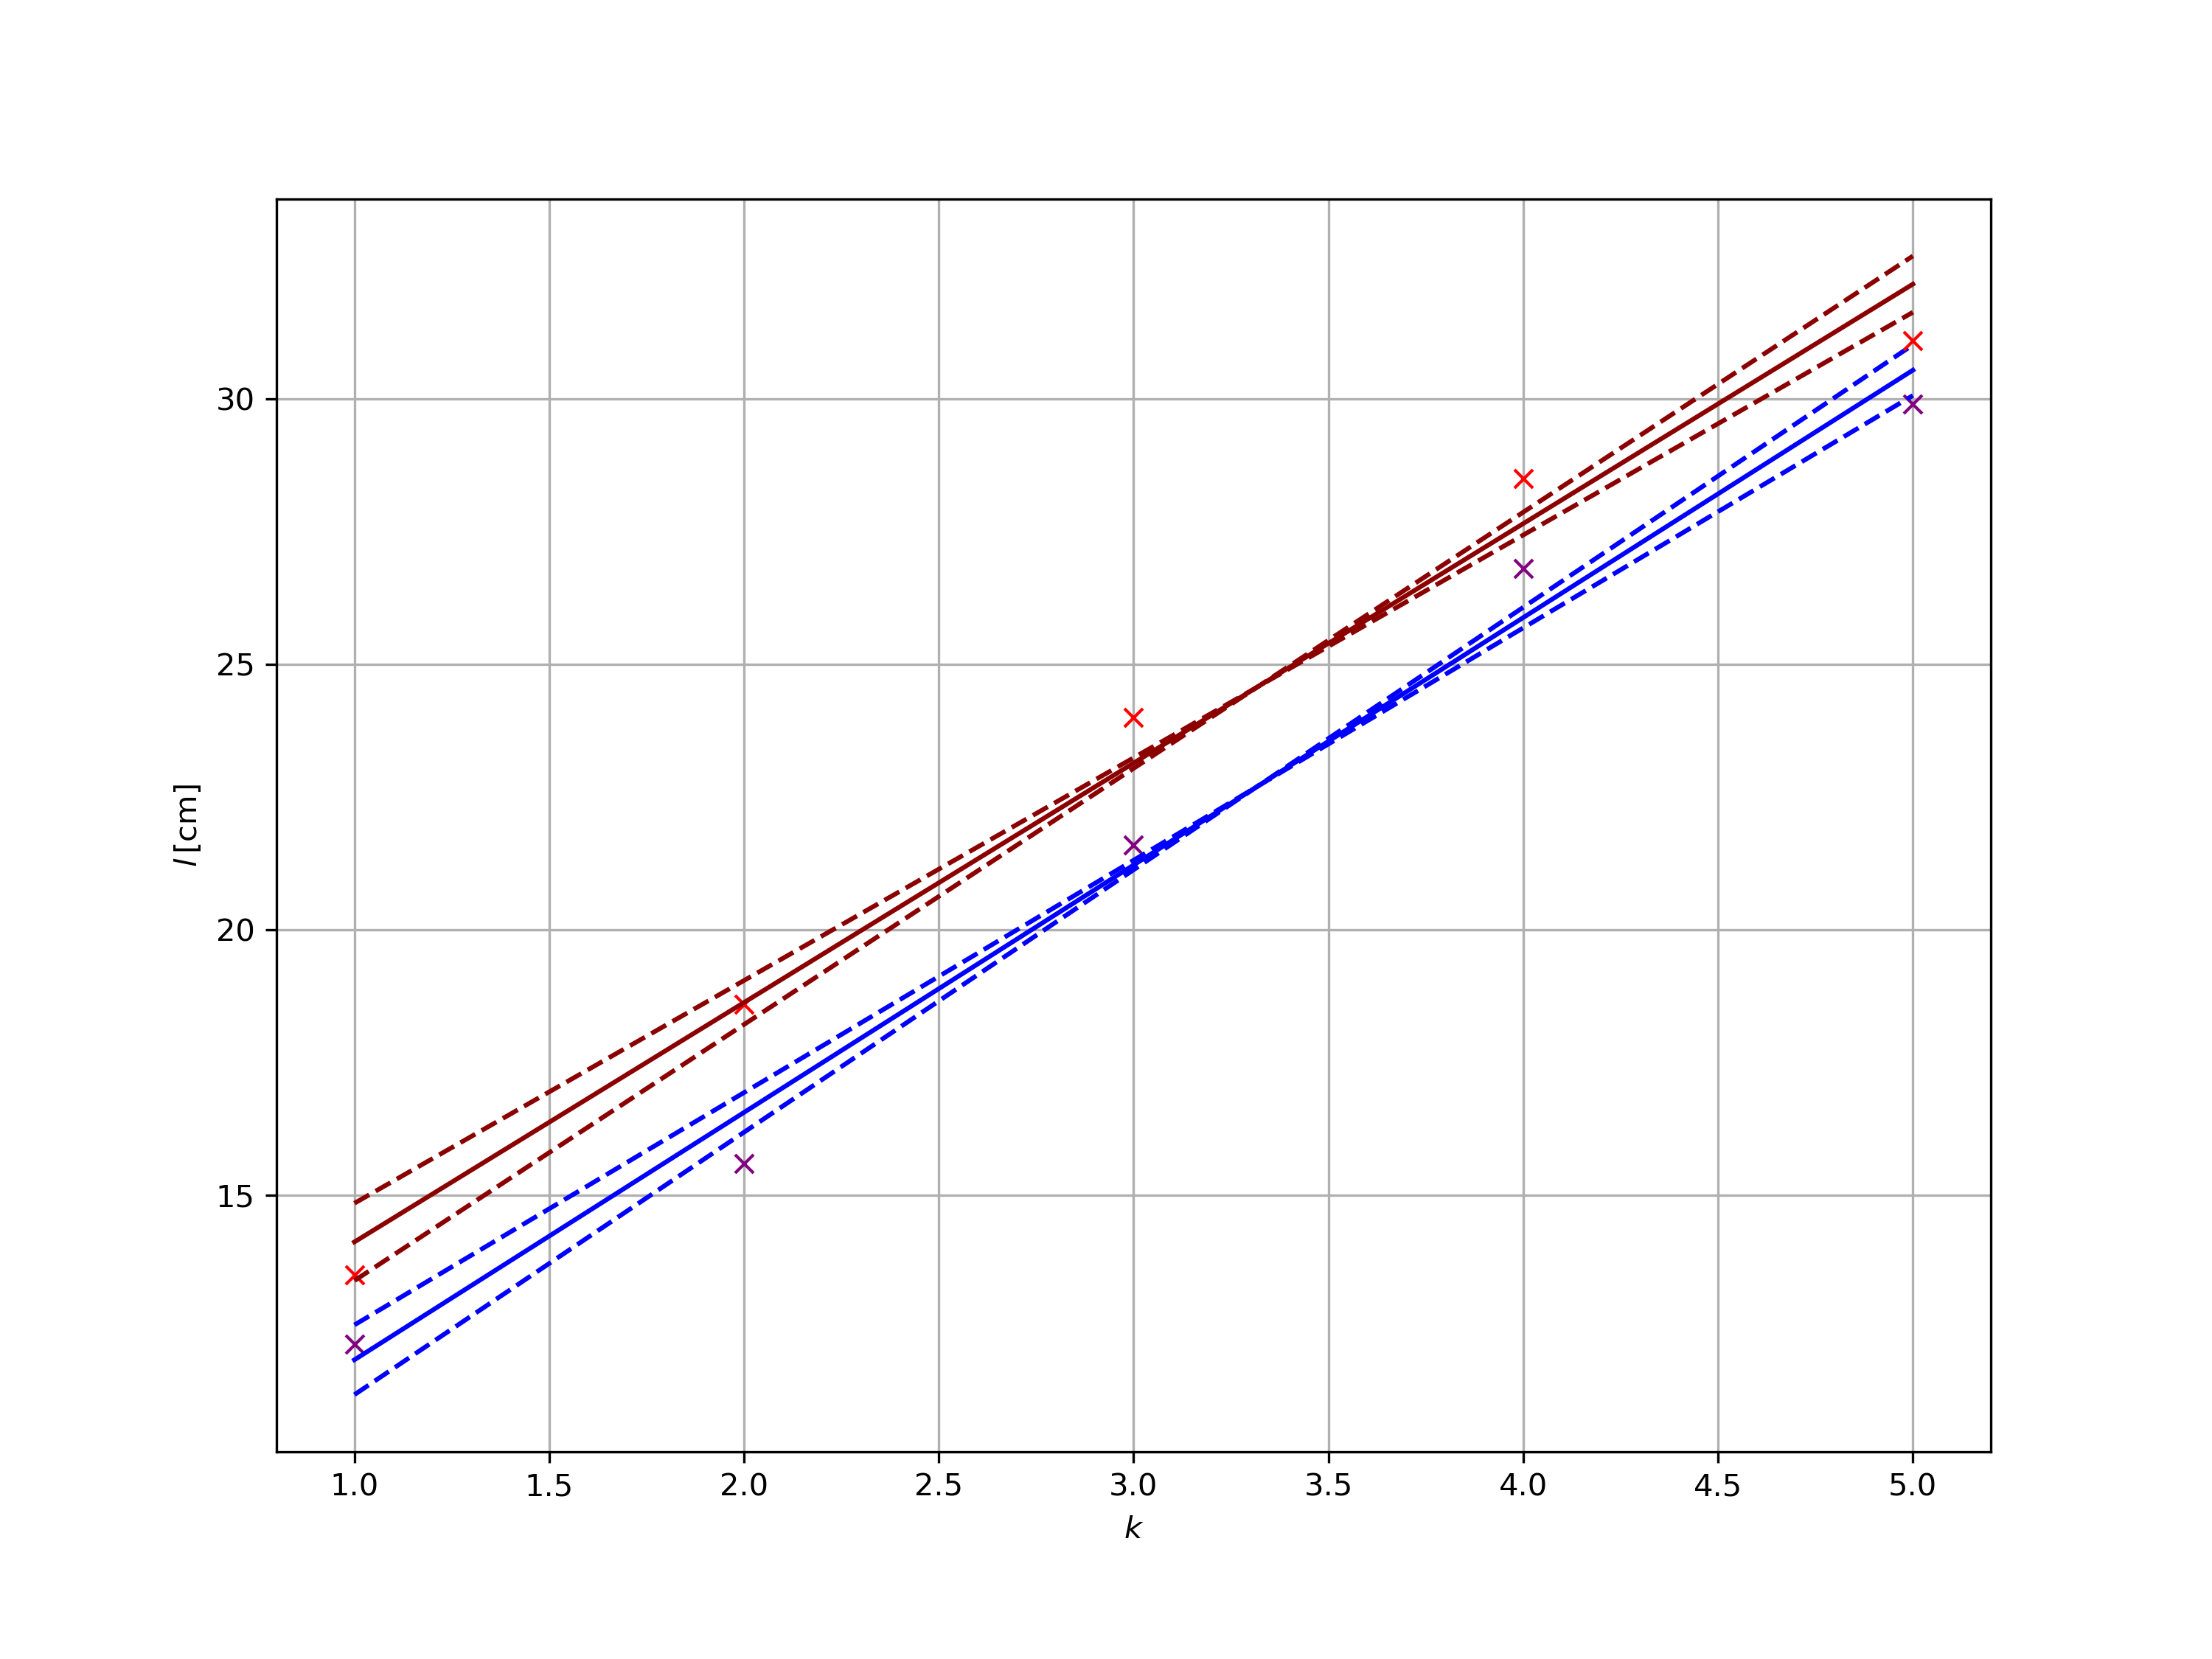
\includegraphics[width=0.8\textwidth]{1firstmeasurementminmax}}
\renewcommand\thefigure{6}
\caption[Auftragen der Maxima und Minima in Abh\"angikeit der Frequenz f\"ur den ersten Versuchsteil bei Frequenz um 5036 Hz]{Auftragen der Maxima und Minima in Abh\"angikeit der Frequenz f\"ur den ersten Versuchsteil bei Frequenz um 5036\,Hz.}
\label{Abb:6}
\end{figure}

\begin{figure}[p]
	\centering
	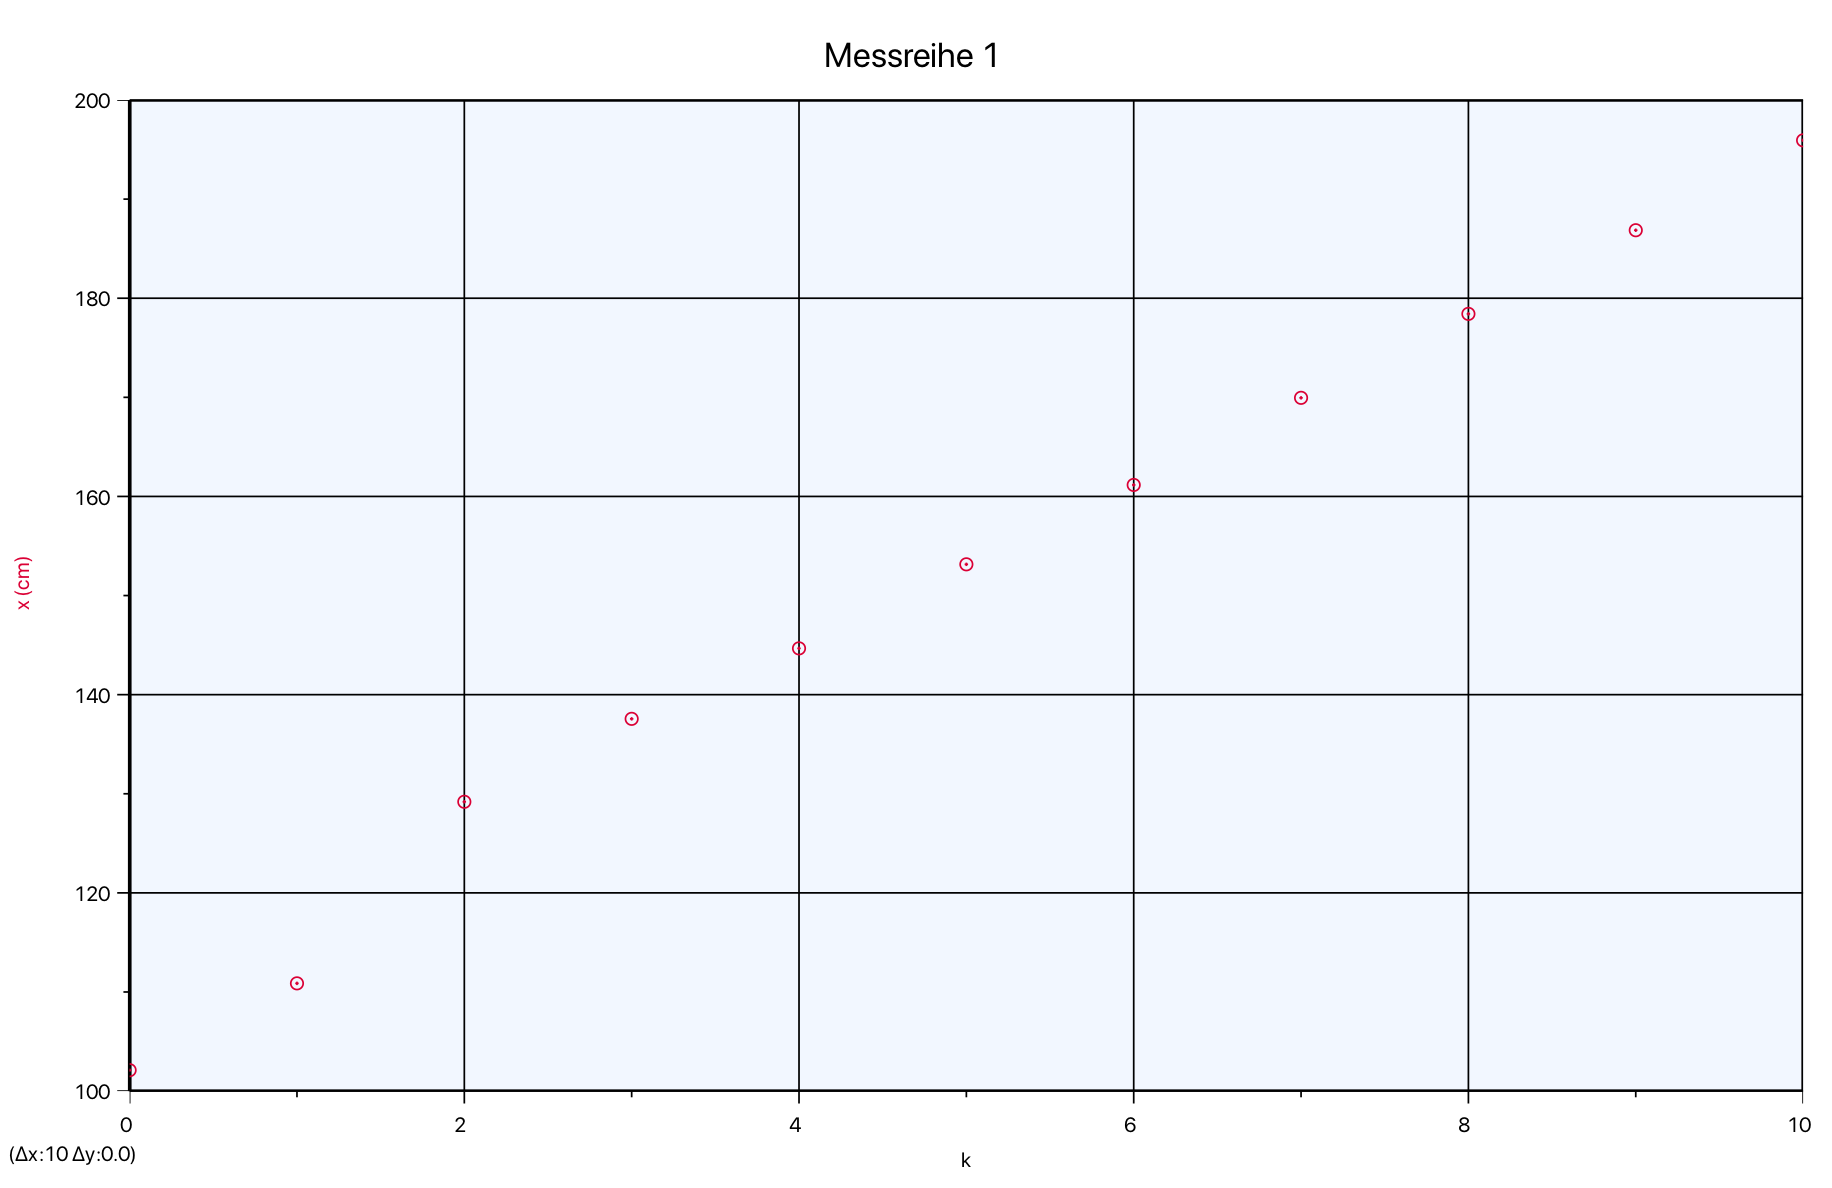
\includegraphics[width=\linewidth]{Anhang1}
	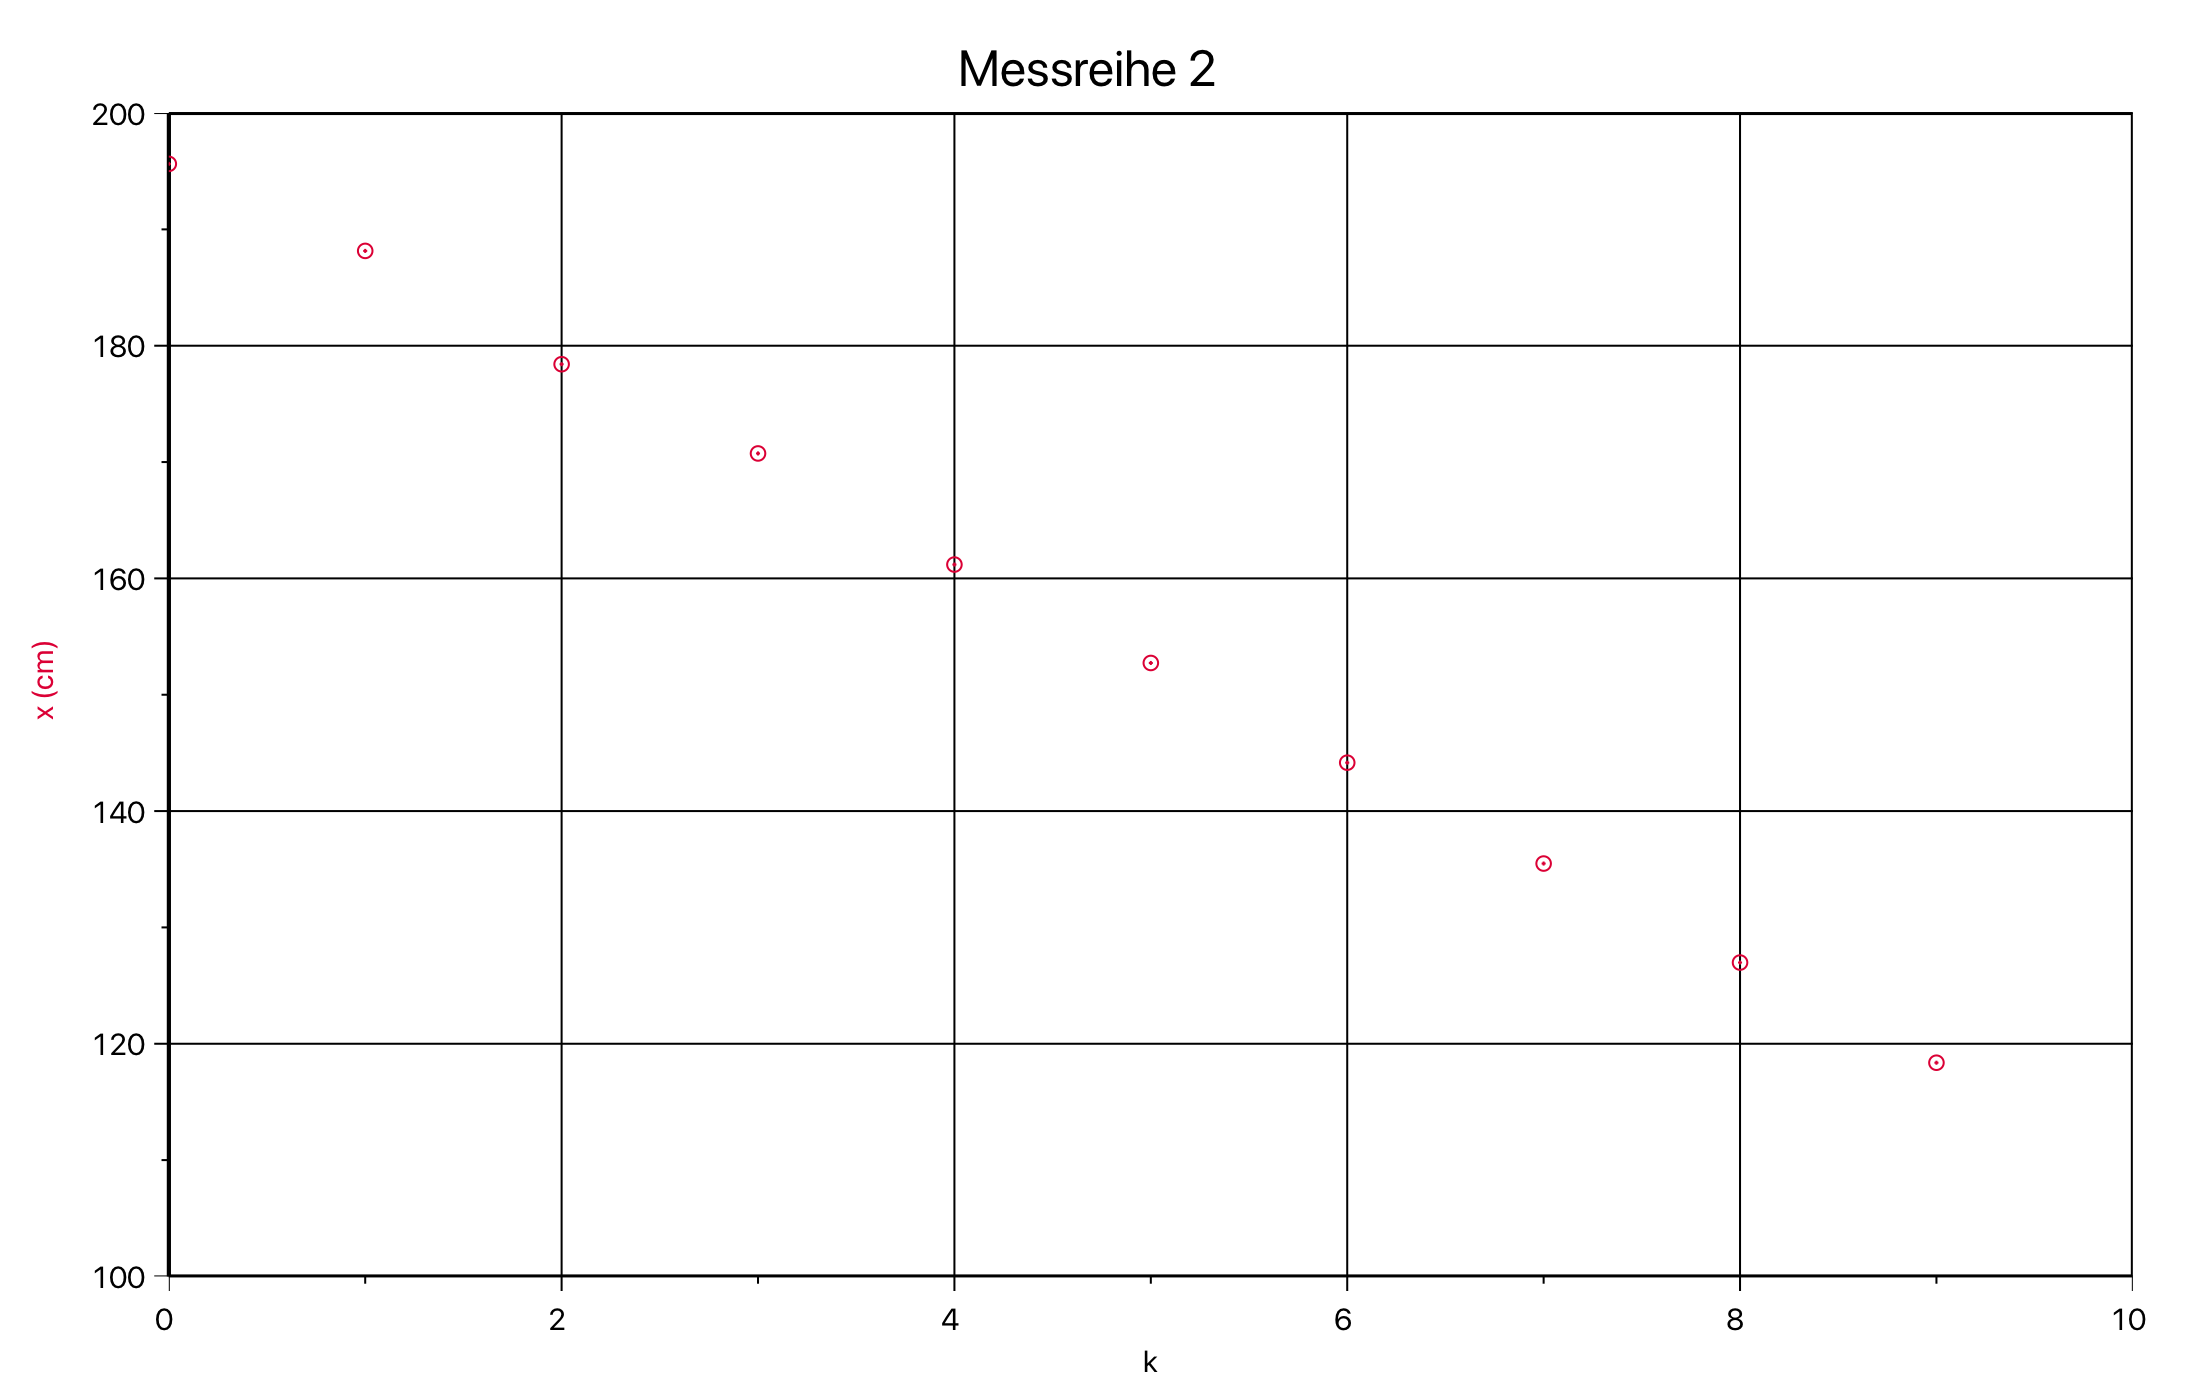
\includegraphics[width=\linewidth]{Anhang2}
	\caption{Der zur Mikrometerschraube relative Position des Empfängers, wo es eine $2\pi$ Phasenverschiebung gab, als Funktion von $k$ (Teil 1). Hier sind die Fehlerbalken zu klein um sie zu erkennen.}
\end{figure}
\begin{figure}
	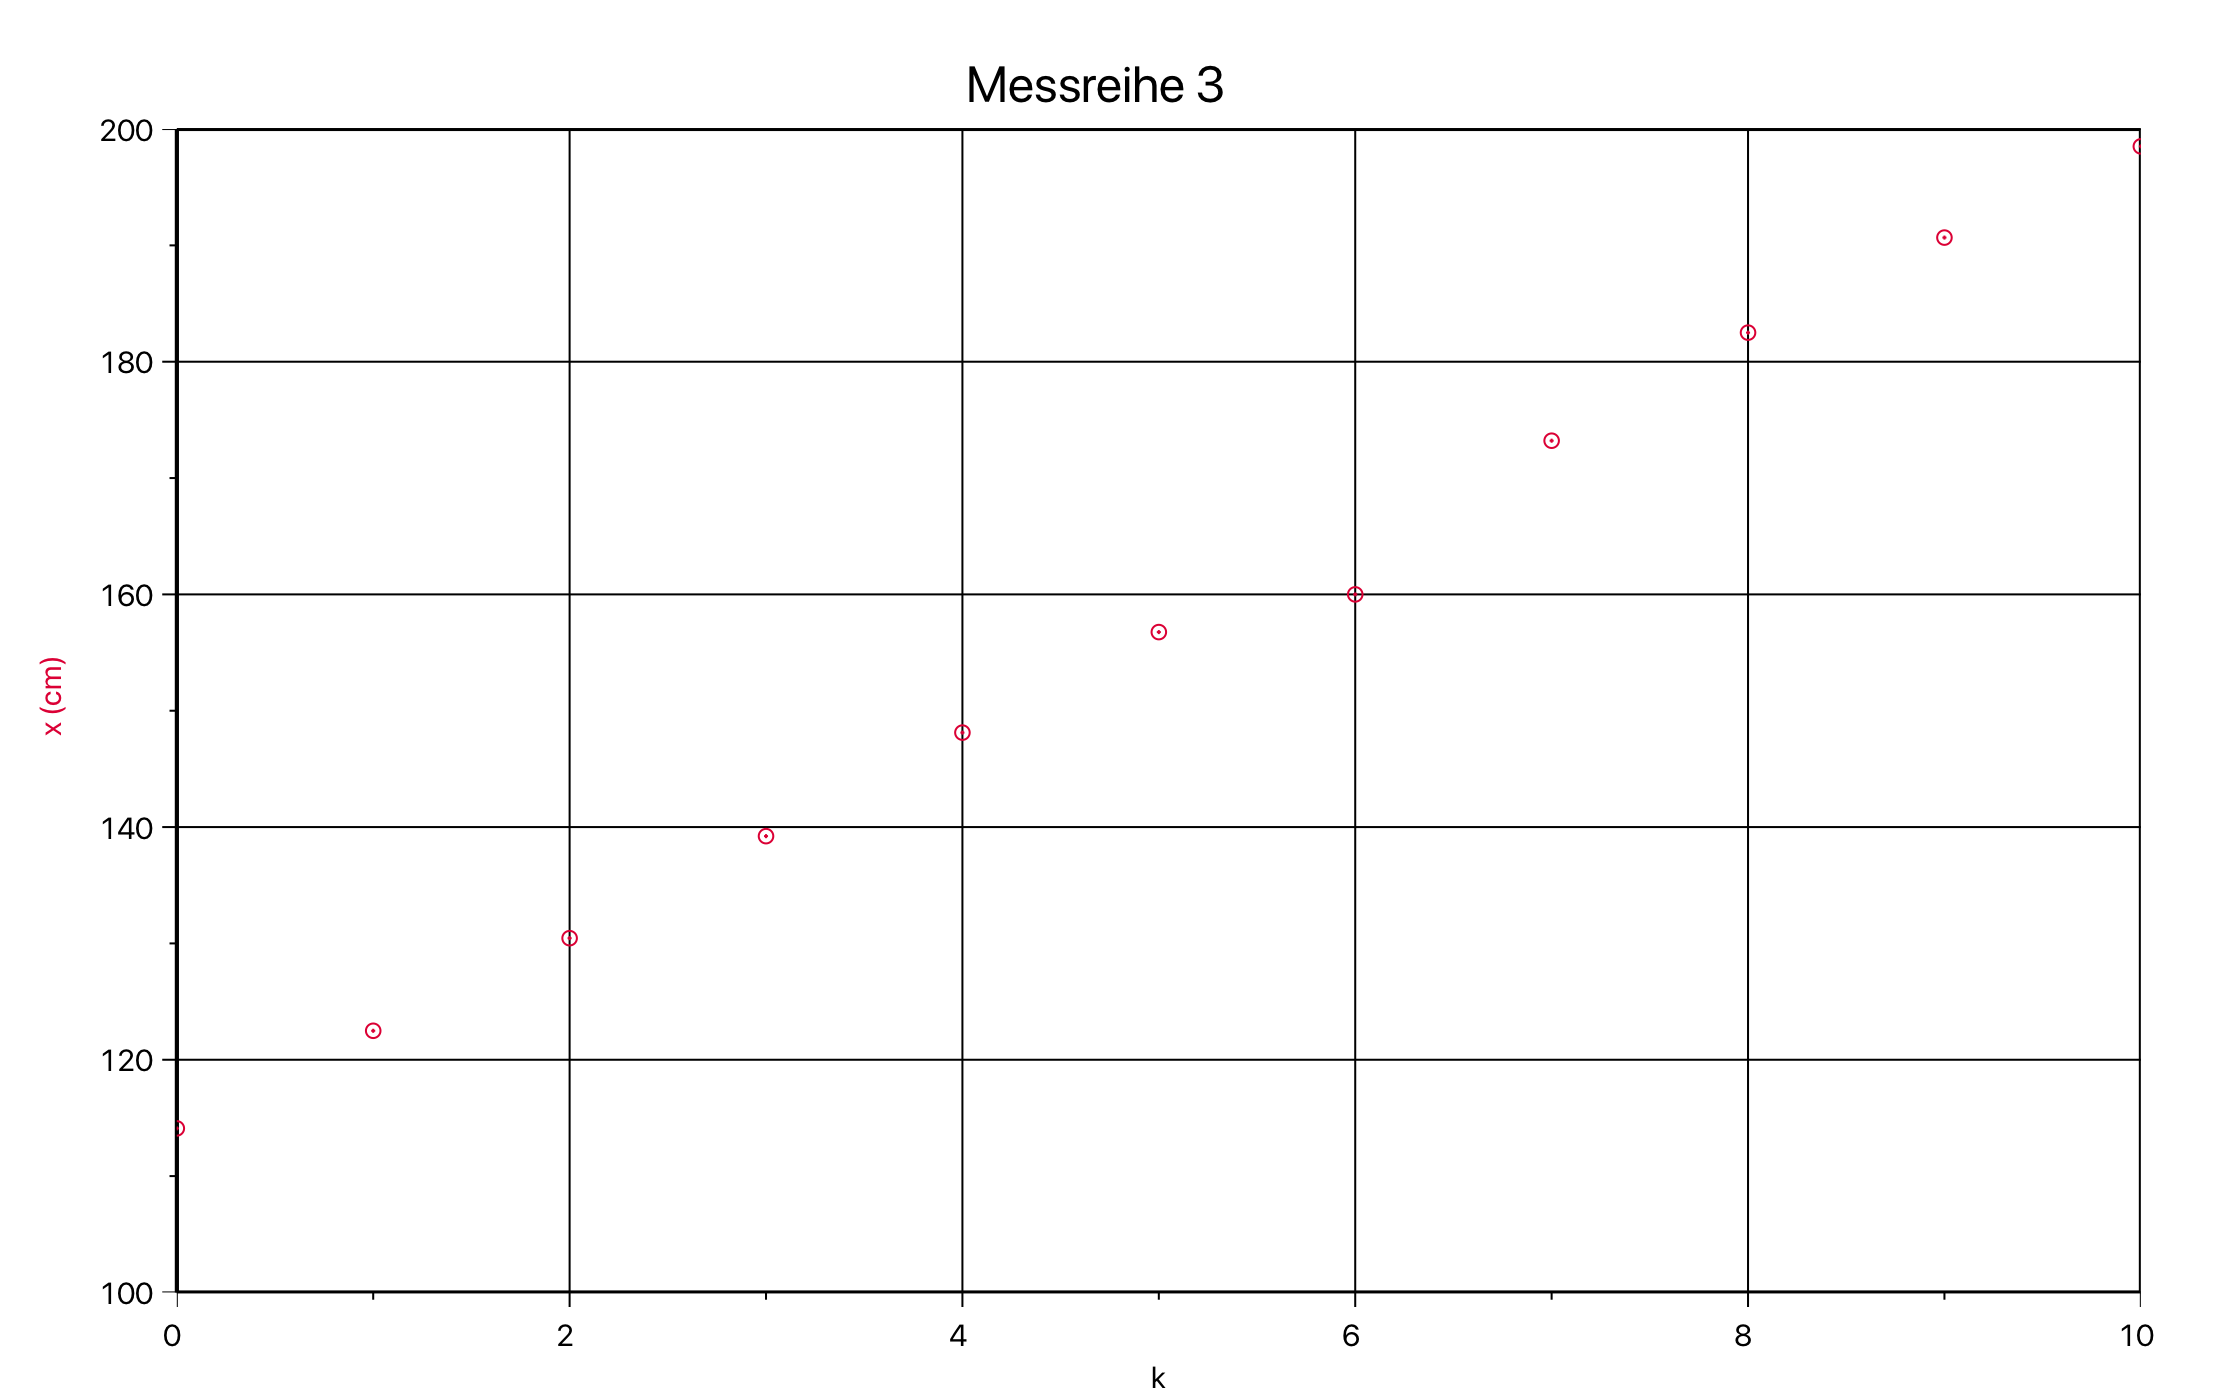
\includegraphics[width=\linewidth]{Anhang3}
	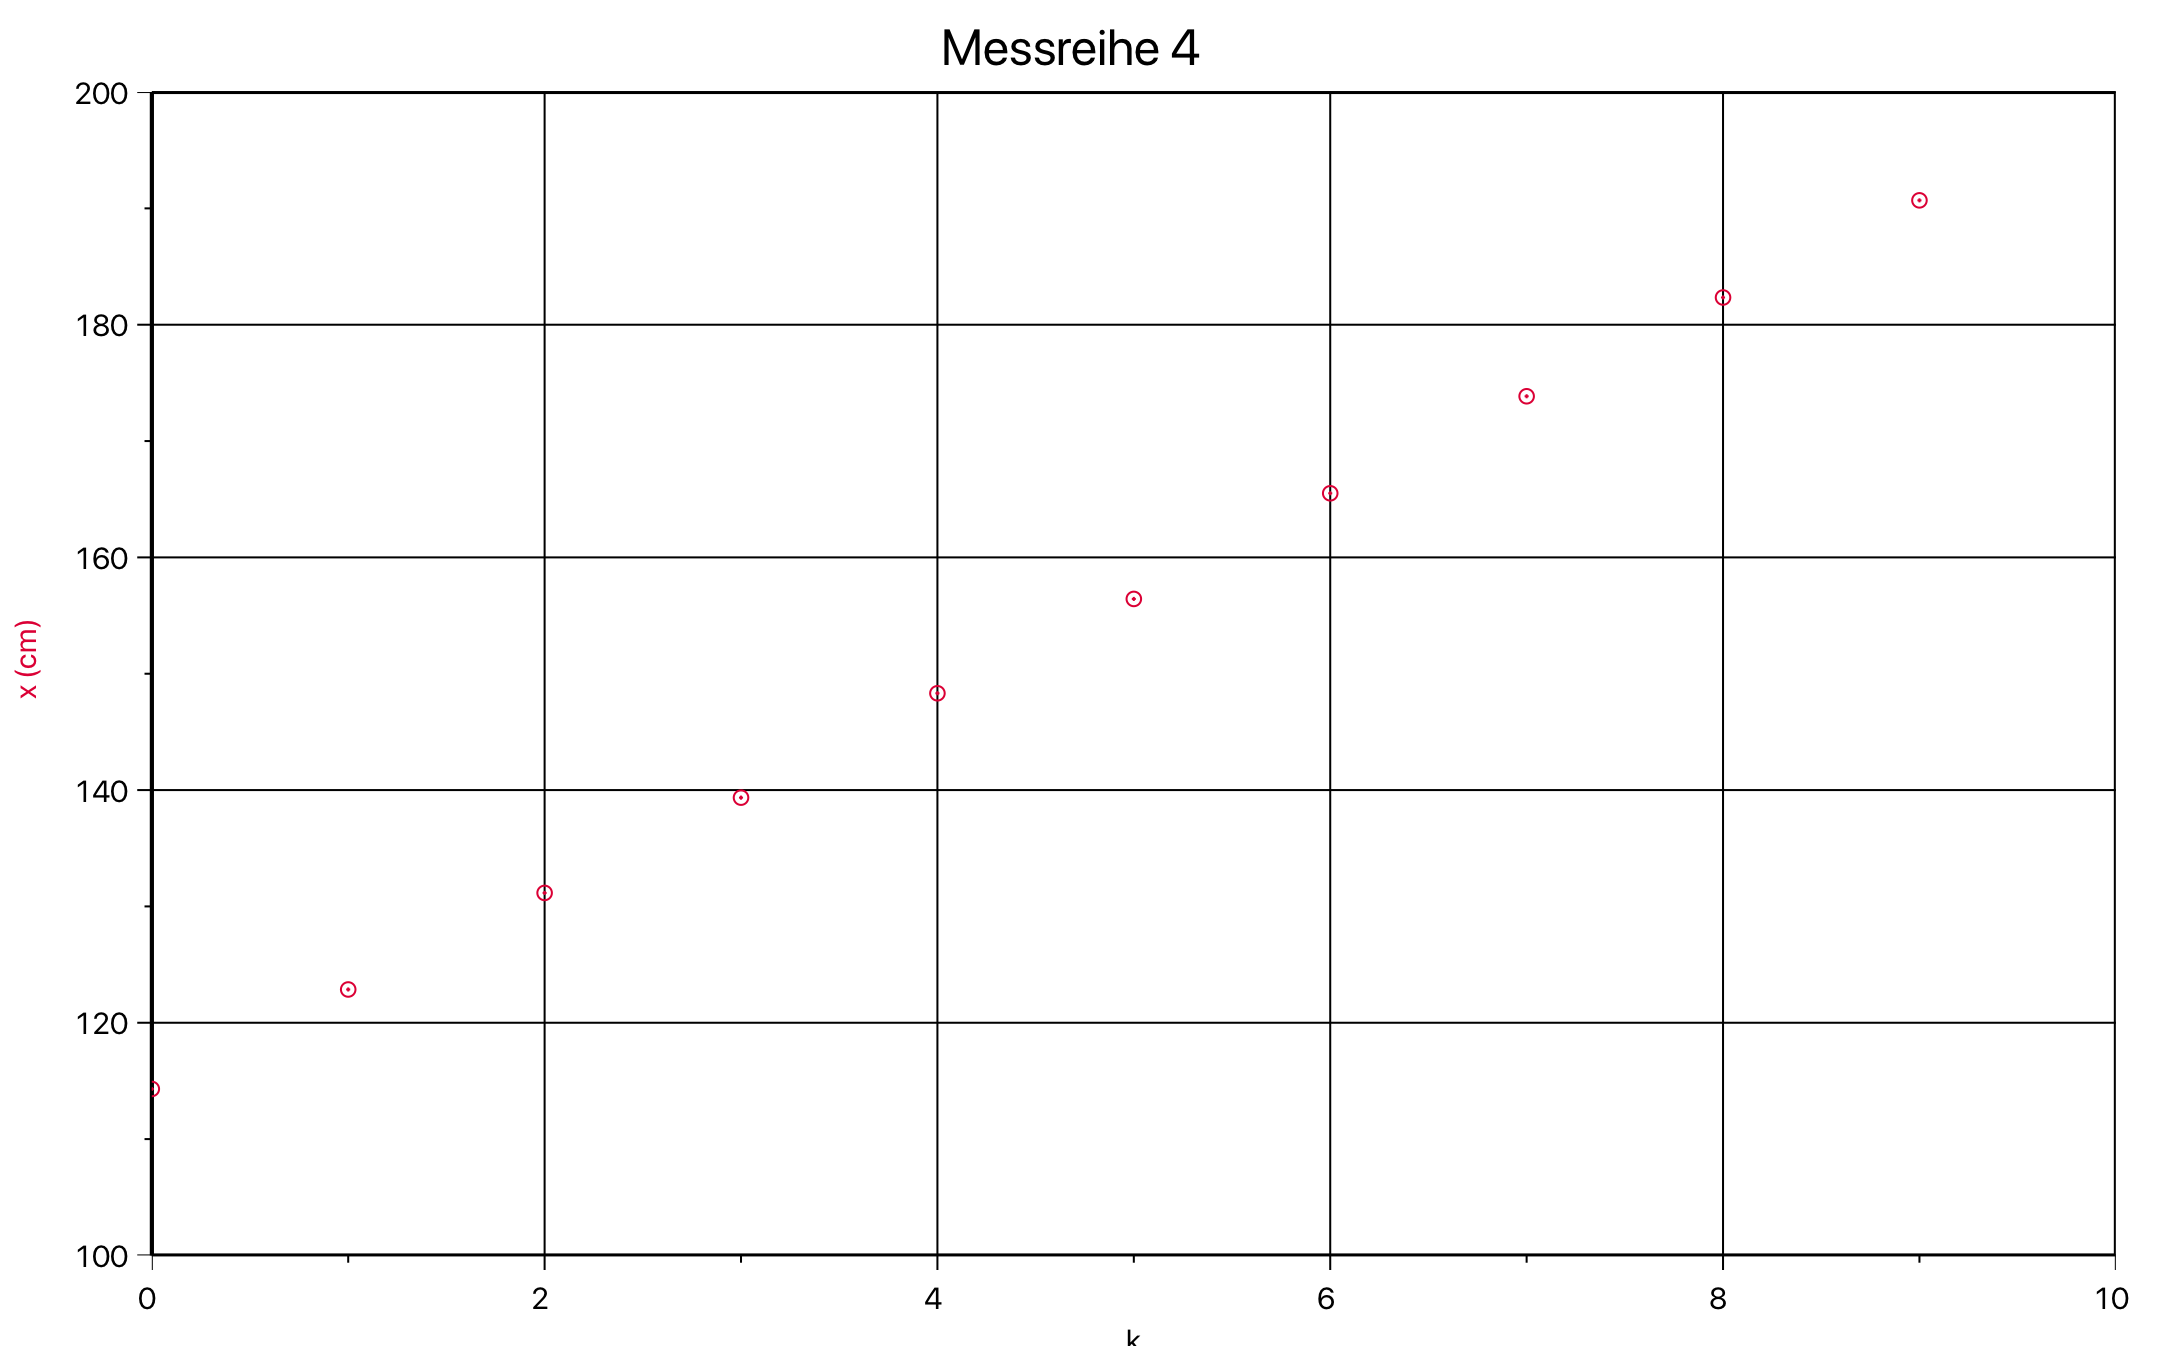
\includegraphics[width=\linewidth]{Anhang4}
	\caption{Der zur Mikrometerschraube relative Position des Empfängers, wo es eine $2\pi$ Phasenverschiebung gab, als Funktion von $k$ (Teil 2). Hier sind die Fehlerbalken zu klein um sie zu erkennen.}
\end{figure}

\begin{figure}[p]
\centering
\fbox{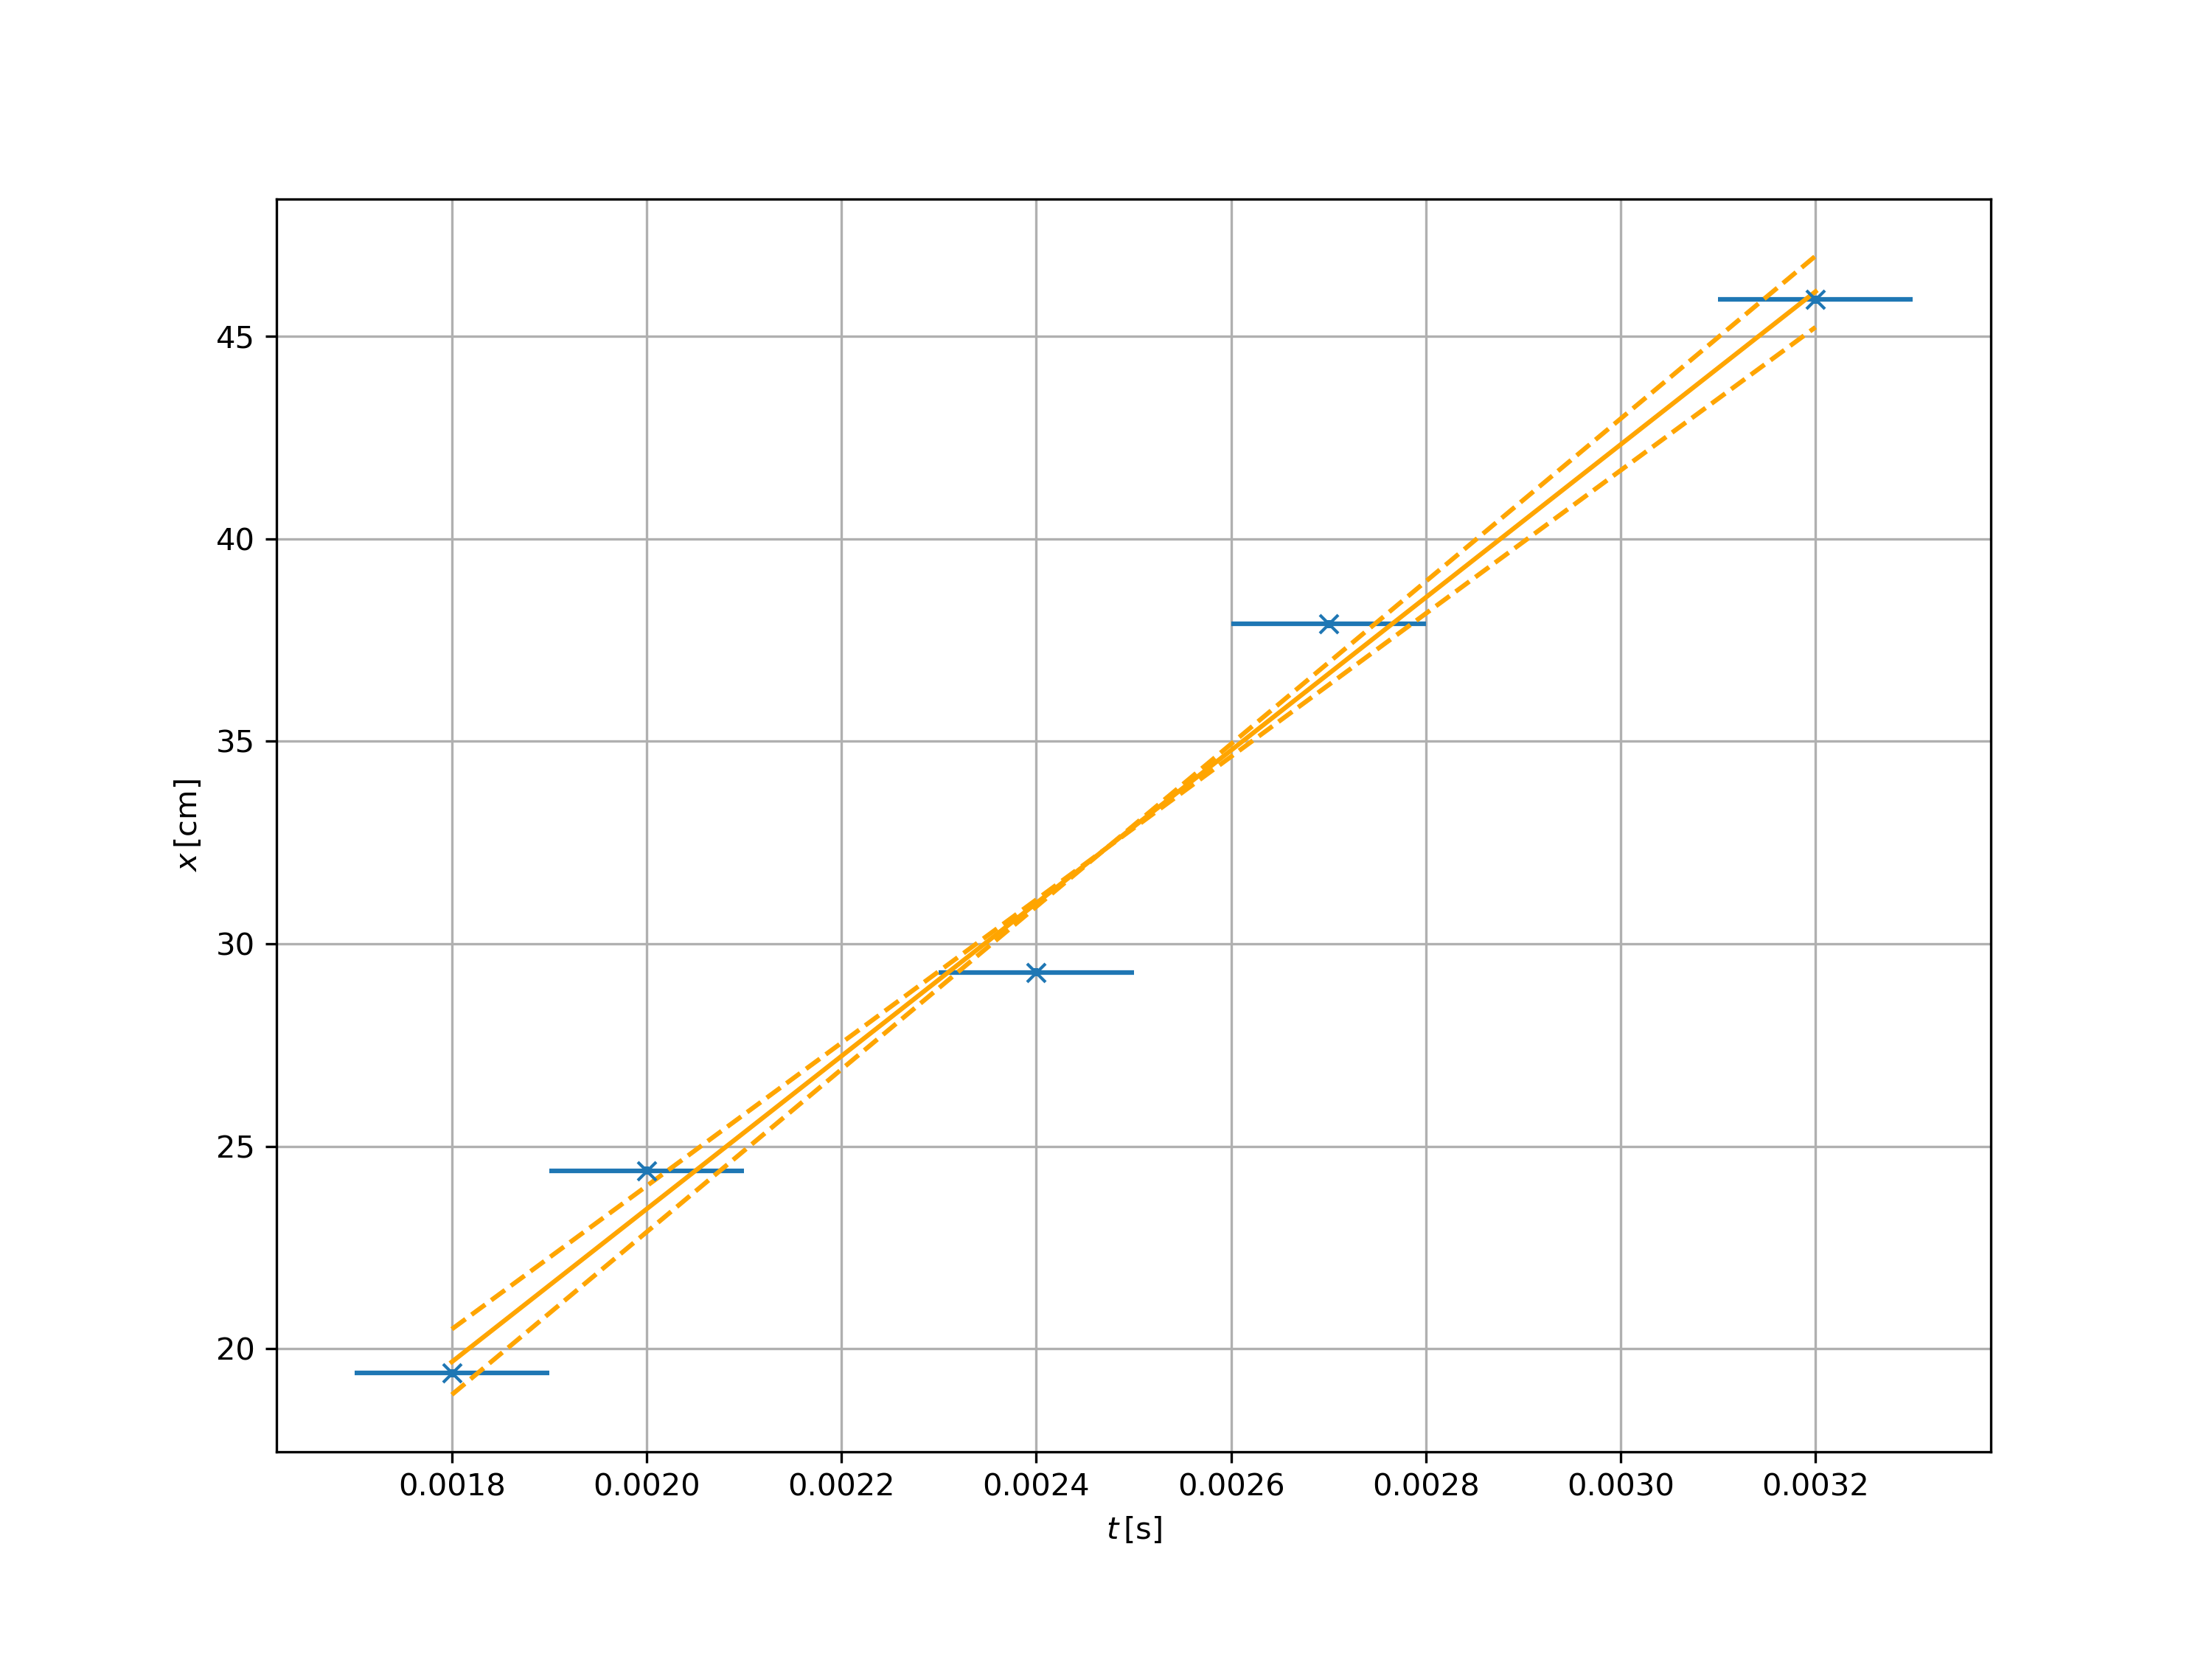
\includegraphics[width=0.8\textwidth]{3xt}}
\renewcommand\thefigure{8}
\caption[Dritter Versuchsteil: Zeit gegen Position mit linearerer Regression]{Dritter Versuchsteil: Zeit gegen Position mit linearerer Regression. Hier sind die Fehlerbalken in $y$ zu klein um sie zu erkennen.}
\label{Abb:8}
\end{figure}

\begin{thebibliography}{9}
%\bibitem{Uncertainties}''Correlations between variables are automatically handled, which sets this module apart from many existing error propagation codes.'' - https://pythonhosted.org/uncertainties/
\bibitem{Anleitung} Physikalisches Institut der Albert-Ludwigs-Universität Freiburg (Hrsg.) (08/2018): Versuchsanleitungen zum Physiklabor für Anfänger*innen, Teil 1, Ferienpraktikum im Sommersemester 2018.
\end{thebibliography}

\end{document}